%% This is file `sample-sigconf.tex',
%% generated with the docstrip utility.
%%
%% The original source files were:
%%
%% samples.dtx  (with options: `sigconf')
%%
%% IMPORTANT NOTICE:
%%
%% For the copyright see the source file.
%%
%% Any modified versions of this file must be renamed
%% with new filenames distinct from sample-sigconf.tex.
%%
%% For distribution of the original source see the terms
%% for copying and modification in the file samples.dtx.
%%
%% This generated file may be distributed as long as the
%% original source files, as listed above, are part of the
%% same distribution. (The sources need not necessarily be
%% in the same archive or directory.)
%%
%%
%% Commands for TeXCount
%TC:macro \cite [option:text,text]
%TC:macro \citep [option:text,text]
%TC:macro \citet [option:text,text]
%TC:envir table 0 1
%TC:envir table* 0 1
%TC:envir tabular [ignore] word
%TC:envir displaymath 0 word
%TC:envir math 0 word
%TC:envir comment 0 0
%%
%%
%% The first command in your LaTeX source must be the \documentclass
%% command.
%%
%% For submission and review of your manuscript please change the
%% command to \documentclass[manuscript, screen, review]{acmart}.
%%
%% When submitting camera ready or to TAPS, please change the command
%% to \documentclass[sigconf]{acmart} or whichever template is required
%% for your publication.
%%
%%
\documentclass[sigconf]{acmart}

\usepackage[most]{tcolorbox}
\usepackage{graphicx}
\usepackage{listings}
\usepackage{xcolor}

\lstset{
    language=Python,
    basicstyle=\ttfamily,
    keywordstyle=\color{blue},
    stringstyle=\color{red},
    commentstyle=\color{green},
    morecomment=[l][\color{magenta}]{\#}
}

%%
%% \BibTeX command to typeset BibTeX logo in the docs
\AtBeginDocument{%
  \providecommand\BibTeX{{%
    Bib\TeX}}}

%% Rights management information.  This information is sent to you
%% when you complete the rights form.  These commands have SAMPLE
%% values in them; it is your responsibility as an author to replace
%% the commands and values with those provided to you when you
%% complete the rights form.
% \copyrightyear{2024}
% \acmYear{2024}
% \setcopyright{rightsretained}

%% These commands are for a PROCEEDINGS abstract or paper.
% \acmConference[NLBSE '24]{2024 ACM/IEEE International Workshop on
% NL-based Software Engineering}{April 20, 2024}{Lisbon, Portugal}
% \acmBooktitle{2024 ACM/IEEE International Workshop on NL-based
% Software Engineering (NLBSE '24), April 20, 2024, Lisbon, Portugal}
% \acmDOI{10.1145/3643787.3648032}
% \acmISBN{979-8-4007-0576-2/24/04}
%%
%%  Uncomment \acmBooktitle if the title of the proceedings is different
%%  from ``Proceedings of ...''!
%%
%%\acmBooktitle{Woodstock '18: ACM Symposium on Neural Gaze Detection,
%%  June 03--05, 2018, Woodstock, NY}
% \acmPrice{15.00}
% \acmISBN{978-1-4503-XXXX-X/18/06}


%%
%% Submission ID.
%% Use this when submitting an article to a sponsored event. You'll
%% receive a unique submission ID from the organizers
%% of the event, and this ID should be used as the parameter to this command.
%%\acmSubmissionID{123-A56-BU3}

%%
%% For managing citations, it is recommended to use bibliography
%% files in BibTeX format.
%%
%% You can then either use BibTeX with the ACM-Reference-Format style,
%% or BibLaTeX with the acmnumeric or acmauthoryear sytles, that include
%% support for advanced citation of software artefact from the
%% biblatex-software package, also separately available on CTAN.
%%
%% Look at the sample-*-biblatex.tex files for templates showcasing
%% the biblatex styles.
%%

%%
%% The majority of ACM publications use numbered citations and
%% references.  The command \citestyle{authoryear} switches to the
%% "author year" style.
%%
%% If you are preparing content for an event
%% sponsored by ACM SIGGRAPH, you must use the "author year" style of
%% citations and references.
%% Uncommenting
%% the next command will enable that style.
%%\citestyle{acmauthoryear}


%%
%% end of the preamble, start of the body of the document source.
\begin{document}

%%
%% The "title" command has an optional parameter,
%% allowing the author to define a "short title" to be used in page headers.
\title{Exploring the Role of Feedback in Developing Machine Learning
Code}

%%
%% The "author" command and its associated commands are used to define
%% the authors and their affiliations.
%% Of note is the shared affiliation of the first two authors, and the
%% "authornote" and "authornotemark" commands
%% used to denote shared contribution to the research.

\author{Arumoy Shome}
\email{a.shome@tudelft.nl}
\affiliation{%
  \institution{Delft University of Technology}
  \country{Netherlands}
}

\author{Lu{\`\i}s Cruz}
\email{l.cruz@tudelft.nl}
\affiliation{%
  \institution{Delft University of Technology}
  \country{Netherlands}}

\author{Diomidis Spinellis}
\email{d.spinellis@tudelft.nl}
\affiliation{%
  \institution{Delft University of Technology}
  \country{Netherlands}
}

\author{Arie van Deursen}
\email{arie.vandeursen@tudelft.nl}
\affiliation{%
  \institution{Delft University of Technology}
  \country{Netherlands}
}

%%
%% The abstract is a short summary of the work to be presented in the
%% article.
\begin{abstract}

\end{abstract}

%%
%% Keywords. The author(s) should pick words that accurately describe
%% the work being presented. Separate the keywords with commas.
% \keywords{SE4AI, NLP4Code, ML Testing, Visualisations, Assertions,
% Computational Notebooks, Automated Tool}

%%
%% This command processes the author and affiliation and title
%% information and builds the first part of the formatted document.
\maketitle

\section{Introduction}

\section{Methodology}

\begin{figure}
  \centering
  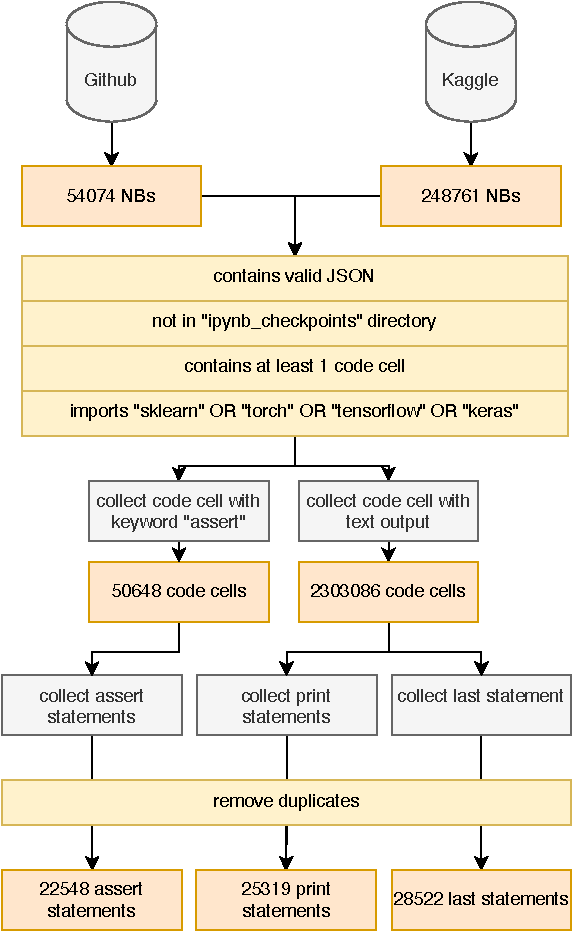
\includegraphics[width=\linewidth]{esem24-method.pdf}
\end{figure}
\section{Results}

% TODO: for each of the feedback types; start with the descriptive and lexical analysis we performed
% TODO: then move into the case studies, and link them to existing literature; use the fault and failure taxonomies; perhaps also link the feedbacks to ML lifecylce proposed by Amershi 2019?

\subsection{Implicit feedback using \texttt{print} statements and output of code cells}

% TODO: why do we check the distribution of the data, particularly during the EDA phase?
\textbf{\emph{Data distribution check (O2, O4, O9, O14, O20, O25, O48)}}

\textbf{\emph{Data relationship check (O6, 010)}} Check if feature is linearly related with the target feature (for linear regression models).

\textbf{\emph{Dependency check (P71, P86)}}. P71 checks that the version of an external library while P86 checks that Cuda is available. 

\textbf{\emph{Execution time check (P66)}}. Print total training time of the model.

% TODO: highlight the use of visualisations to check for missing values; what is the benefit of using a visualisation instead of code?
\textbf{\emph{Missing value check (O12, O36, P74)}}. Check if missing values are present in any features of the data. After loading the dataset and in the EDA phase of analysis.

\textbf{\emph{Model performance check (O3, O50, O52, O57, O74, P3, P6, P8--12, P16--19, P23, P24, P28, P30, P34, P42, P47, P48, P50, P51, P54, P55, P57, P58, P61, P78, P93)}}. Check various performance metrics of models on the test set. Typically, the classification report is used. Precision and recall is checked using the confusion matrix. Residuals of a linear model is checked.

\textbf{\emph{Model architecture (P92)}}. Print the architecture of the neural network. The layers of the model, neurons in each layer and the activation functions are printed in a text diagram.

\textbf{\emph{Resource check (O64, O66, P68, P82, P107)}}. Check is GPU or TPU resources are available. We suspect these checks are coming from Google Colab notebooks where computation can be off-loaded to remote hardware. In P107, check that the pre-trained model was successfully loaded from the file system.

\textbf{\emph{Shape check (P4, P32, P117)}}. Check the number of examples in the test data; check shape of training data; check shape of training labels.

\textbf{\emph{Type check (O71, P43)}}. Check that the data type of the features in the training set 

% NOTE: perhaps these are spot-checks?
\textbf{\emph{Value check (O56, O60, P64, P67, P114)}}. Check that one-hot encoding worked; manually verify the output of an activation function in a neural network against expected value.

\textbf{\emph{Model training (O8, O31, O42, P77)}}. Periodically print the progress made in training by printing the training loss/accuracy of model.

\subsection{Explicit feedback using \texttt{assert} statements}

% TODO: find out more about batch training
\textbf{\emph{Batch size check (A21, A28, A70)}}. Neural Networks are trained using smaller batches that makes it more efficient use of hardware GPU cores. We encounter assertions that check the size of the batch prior to training or prior to calculating the score of the NN.

\textbf{\emph{Data leakage check (A33)}}. It is a best practise to ensure that the ML model is not tested using examples that it has already encountered during training. This is to ensure that the model is not overfitting on the training data and is able to generalise to examples similar to the distribution of the training set, but not exactly the same. In A33 we see that the assert ensures that the training and validation sets do not share any examples.

% TODO: what is the motivation of this assertion? Find prior work on
% python dependency management?
\textbf{\emph{Dependency check (A18, A67)}}. This is a unique type of test which occurs due to the unique workflow of notebooks. Typically dependencies are managed through external means such as dedicated dependency management solutions or the builtin Python method using a requirements.txt file. We notice assertions that check that the major version of an external dependency is equal to the specified value.

% NOTE: missing-value-check and existence-check

\textbf{\emph{Existence check (A86)}}. Existence checks are carried out in various contexts. Most are for checking that columns in a dataset do not contain missing values. Others ensure that certain columns (such as the column containing the labels of the data) exists in the dataset prior to splitting the data into training and testing sets. Existence checks are frequently performed after data pro-processing  steps are performed to ensure that missing values were not added to the dataset.

% TODO: we need to elaborate this one with examples 

\textbf{\emph{Mathematical property checks (A3, A25, A56, A64)}}. Machine learning models are often rooted in statistical models. Implementing neural networks requires a graph of linear algebra and matrix multiplication. We find several assertions that test the mathematical properties of arrays and matrices after performing matrix operations.

% TODO: there is a lot to discuss here, bring in the discussion on the
% use of comparison operators and such into the mix here

\textbf{\emph{Model performance check (A7, A15, A19, A22, A24, A26, A38, A54, A58, A59, A72)}}. We see several assertions that test for the performance of the trained ML model against a validation or test test. The assertions often compare a performance metric (such as accuracy, precision, recall, F1, etc) against a predefined threshold.

% TODO: this needs more work and investigation
\textbf{\emph{Network architecture check (A11)}}. We only have one example here.

% TODO lots to elaborate and discuss here
\textbf{\emph{Resource check (A10, A14, A37, A60, A74)}}. We find assertions that check that a pre-trained model exists on the file system, or that data can be loaded from a specified file path. There are also checks that ensure that a visualisation created using matplotlib contains data in it.

\textbf{\emph{Data shape check (A5, A9, A13, A16, A17, A29, A31, A61, A71, A76--78, A82, A84, A85, A89, A90, A91, A93--96, A98--101)}}. ``Swiss army knife'' of assertions!

\textbf{\emph{Type check (A2, A35, A40, A81, A88)}}. Checking the data type of features and such.

\textbf{\emph{Value check (A30, A41, A44--46, A52, A65, A68, A69, A73, A92)}}. Check that the values in a column are in the specified values (categorical) or in a specified range (normalised continuous variable) or binary (such as the label column).

% NOTE: blanks and unit-tests
\textbf{\emph{Miscellaneous checks (A6, A20, A32, A34, A36, A53, A62, A75, A83, A87, A97)}}. These feel like unit tests, performed in lieu of writing full test suites in the notebook.

\bibliographystyle{ACM-Reference-Format} \bibliography{bibliography}
\end{document}
\endinput
%%
%% End of file `sample-sigconf.tex'.
